% !TeX encoding=utf8
% !TeX spellcheck=de-DE
% !TeX root=../UID_Project_Documentation.tex

\section{Prototyping}

\subsection{Entwicklung des Prototypen}

Aus den verschiedenen Ideen die durch die Sketches aufgezeigt wurden, wurde dann der Prototyp entwickelt. Uns war wichtig das der Gulf of Execution und Gulf of Evaluation konsistent sind und die Benutzer der Anwendung durch unvorhersehbares Verhalten verwirren oder sogar frustrieren. Wir haben uns bei dem Prototyp für eine Android App entschieden, da aufgrund der Marktanalyse Smartphone Apps für Online Nachrichten den größten Marktanteil haben. Android aus dem Grund, da Android für uns eine bekannte Umgebung ist und mittlerweile den größten Marktanteil hat. Diese Entscheidung könnte aber auch zu Nachteilen bei den User Tests führen, falls die Testpersonen des User Test iPhone Benutzer sind.

Die App hat einen Hauptbereich in dem die Haupt Funktionalität angesiedelt ist. In diesem Bereich geht es nur um die Nachrichten, das Erkunden und die \enquote{Feeds}, welche den Kern der App darstellen. Die Navigation funktioniert über eine Tab-Leiste, welche immer sichtbar ist.

Bewusst Abgetrennt sind die persönlichen Daten des Benutzers, die sich über das \enquote{Burger}-Menü öffnen lassen. Von diesem Menü kann der Benutzer zu verschiedenen Übersichten Navigieren, die beispielsweise die abgeschlossenen Abonnements anzeigen. Durch diese Anordnung wollten wir verdeutlichen, das es sich eher um sekundäre Funktionen handelt, die nichts mit den eigentlichen Nachrichten zu tun hat. Diese Gestaltung basiert auf Sketch 3 in Abbildung \ref{fig:sketch-03}.

Die Home Ansicht zeigt einen Default-Feed an, der aus den eigenen Feeds ausgewählt werden kann. Hier werden die Nachrichten jeweils mit Bild und der Schlagzeile angezeigt. Die Nachrichten sollen in einer möglich kurzen Form präsentiert werden. Es wäre auch möglich dies ohne das Bild zu einer Nachricht zu machen, aber da Menschen primär den Sehsinn verwenden, war unseres Erachtens nach die Variante mit Bild und Schlagzeile angenehmer als nur Text. Die Gestaltung dieser Ansicht basiert auf Sketch 2 in Abbildung \ref{fig:sketch-02}.

In der Customize Ansicht werden alle Feeds aufgelistet und es gibt die Möglichkeit einen neuen Feed anzulegen. Das Anlegen der Feeds wird über einen sogenannten \enquote{Floating-Action-Button} angestoßen. Wir haben uns dafür entschieden dies so zu realisieren, da es unserer Ansicht nach deutlich signalisiert, das dieser Button dort ist, um etwas neues anzulegen. Viele Android Apps, unter anderem WhatsApp, gehen einen ähnlichen Weg, wenn es darum geht neue Inhalte anzulegen. Die tatsächliche Ansicht zur Anpassung der Feeds wird mit einem Klick auf das jeweilige Listen Item geöffnet. Die Grundidee für dieses Ansicht lieferte Sketch 4 in Abbildung \ref{fig:sketch-04}. Es wurde in abgewandelter Form die Auflistung übernommen.

Bei dem Konfigurieren oder Erstellen eines neuen Inhalts wird eine Übersicht der vorhandenen digitalen Nachrichtenangebote angezeigt. Ein Checkbox bei jedem Nachrichtenangebot signalisiert, ob diese Quelle für den aktuellen Feed ausgewählt wurde. Ein Schloss-Piktogramm bei dem Item neben der Checkbox signalisiert, dass es sich um einen nicht erworbenen, kostenpflichtigen Anbieter handelt. Wir haben uns an der Stelle für ein Piktogramm anstatt Text entschieden, da wir denken, dass Benutzer so schneller den Sachverhalt wahrnehmen und auch die Gestaltung übersichtlicher ist. Durch einen Klick auf den Nachrichtenanbieter wird eine Übersicht der Kategorien angezeigt, die ein Nachrichtenanbieter anbietet. Ebenso wie der Anbieter übersicht ist eine Checkbox der Indikator zur Auswahl und ein Schloss-Piktogramm signalisiert kostenpflichtige Inhalte. Wenn ein Benutzer kostenpflichtige Inhalte hinzufügt, muss er noch den Kauf bestätigen. Dies geschieht durch ein Popup, welches dem Benutzer zeigen soll, was er/sie mit seiner Handlung verursacht und welche Konsequenzen es hat. Dies geschieht in dem Hinblick Gulf of Execution und Gulf of Evaluation zusammenzubringen. Wir haben uns für diese zweistufige Auswahl der Inhalte entschieden, da es unser Erachtens so den Benutzern eine gute, nicht überladene Übersicht gibt. Mehr Funktionalität, oder ausklappbare Inhalte könnten unerfahrene Benutzer verwirren. Am unteren Rand der View ist ein Button zum speichern, welcher farblich gegenüber den Listen Items abgehoben ist. Seine Funktionalität ist das Speichern. Es soll durch die andere Farbe verdeutlicht werden, dass der Benutzer durch Interaktion mit dem Button die Ansicht verlässt und zur vorherigen Ansicht zurückkehrt und die Daten gespeichert werden.

Die Explore Ansicht dient zur Erkundung von neuen Inhalten und soll bei den Benutzern das Interesse wecken kostenpflichtige Inhalte zu abonnieren. Die Grundidee kommt aus Sketch 3 in Abbildung \ref{fig:sketch-03}. Außerdem orientiert sich die Gestaltung an der Tinder App. Wir haben das Konzept von Tinder abgewandelt, da Nachrichten unseres erachtens nach eine etwas andere Darstellung brauchen als Personen in einer Dating App. Es gibt einen Button zum Anzeigen des aktuellen Artikels und einen Button zum anzeigen des nächsten Artikels. Die Button unterscheiden sich farblich von einander, um die Funktionalität visuell abzugrenzen. In dieser Übersicht werden von der Nachricht grundlegende Informationen angezeigt: Bild, Schlagzeile, Zeitung/Quelle, Resort. Ähnlich wie bei der Home Ansicht war der Gedanke hierbei die Nachricht zu kurz wie möglich zu präsentieren. Die Gestaltung einer Vollbild Ansicht einer einzigen Nachricht wurde gewählt, da es bei der Explore Ansicht explizit um das erkunden einzelner neuer Inhalte für den Benutzer geht. Der Benutzer soll sich dadurch auch die Zeit nehmen und von nichts anderem abgelenkt werden, wenn sich ein Nutzer neue Inhalte anschaut. Wenn der Benutzer sich dazu entscheidet einen Artikel zu lesen, kann er am Ende des Artikels die Quelle mit der Kategorie zu einem seiner Feeds mit einem Button hinzufügen.

Generell haben wir also sehr viel Wert darauf gelegt, die App übersichtlich und leicht benutzbar zu gestalten, sodass auch Personen, die weniger souverän im Umgang mit Smartphones sind, also unserer Persona \enquote{Uli} ähnlich sind, nicht überfordert oder sogar frustriert werden. Dabei wollten wir aber nicht schnellere User (also technikaffine Personen, die der Persona \enquote{Sabine} ähneln) durch unnötig viele Unterbrechungen in Form von Popups oder ähnlichem ausbremsen, sondern diese nur dort einbauen, wo es sinnvoll ist, nämlich wenn zahlungspflichtige Käufe getätigt werden. Dieser Art von Benutzern sollte die Bedienung der App zudem ohnehin leicht fallen, da wir uns an den typischen Android-Design-Paradigmen orientiert haben.

\subsection{Flow Chart}

\begin{figure}[H]
  \centering
  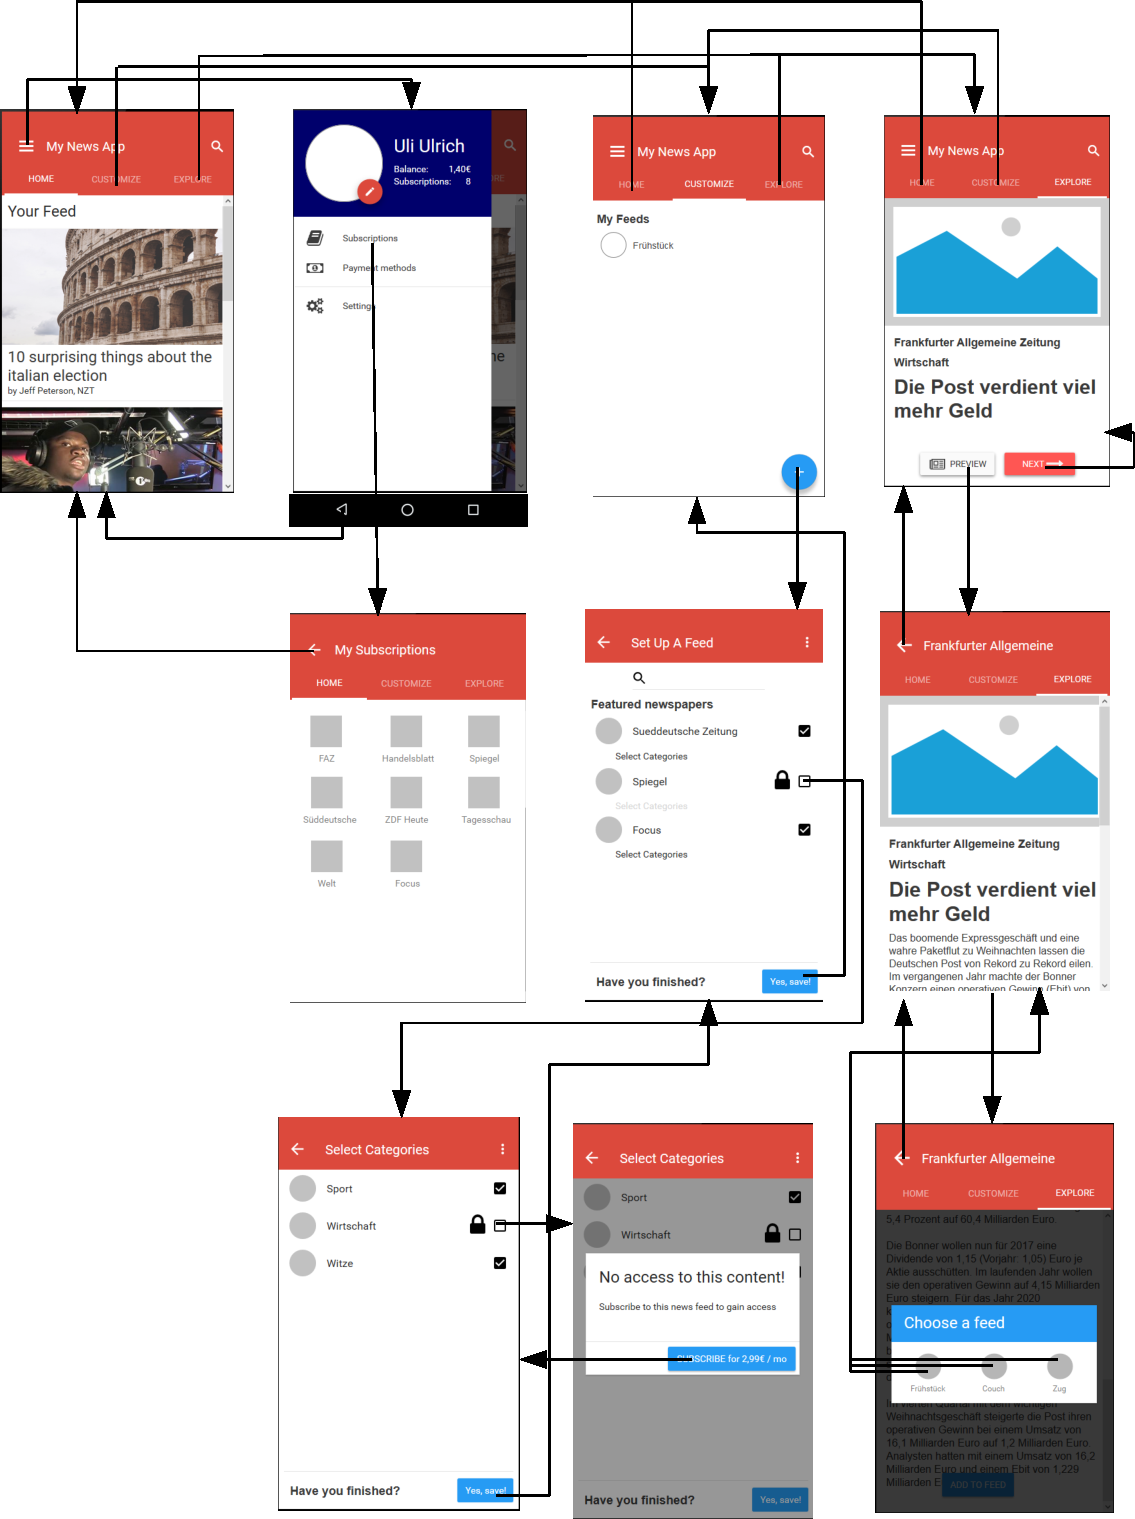
\includegraphics[width=\textwidth]{flowchart}
  \caption{Flowchart der MyNewsApp}
  \label{fig:flowchart}
\end{figure}
